\section{Classificação e etapas da pesquisa}
\label{natureza}

A elaboração do presente estudo caracterizou-se como uma pesquisa aplicada quanto à sua natureza. Segundo \citeonline{silva2005pesquisa}, a pesquisa aplicada visa gerar conhecimentos para aplicação prática e voltados à solução de problemas específicos e interesses locais.

Do ponto de vista da abordagem do problema a pesquisa classifica-se como qualitativa. Para \citeonline{silva2005pesquisa}, a pesquisa qualitativa preocupa-se com o processo de investigação, sendo que há uma relação dinâmica entre o objeto a ser estudado e o sujeito, estabelecendo-se um vínculo indispensável entre o mundo objetivo e a subjetividade do sujeito. Somada a essa questão, destaca-se que a interpretação dos fenômenos e a atribuição de significados pelo pesquisador é o instrumento-chave da pesquisa qualitativa.

Em relação aos objetivos, a pesquisa é exploratória, pois buscou:

\begin{citacao}
proporcionar maior familiaridade com o problema, com vistas a torná-lo mais explícito ou a constituir hipóteses[...] seu planejamento é, portanto, bastante flexível, de modo que possibilite a consideração dos mais variados aspectos relativos ao fato estudado \cite[p. 41]{gil2002elaborar}.
\end{citacao}

No que concerne aos procedimentos técnicos utilizou-se para o presente estudo: a pesquisa bibliográfica, a documental e o estudo de caso \cite{gil2002elaborar}. Esses procedimentos técnicos referem-se à:

\begin{enumerate}
    \item[a)] Pesquisa bibliográfica: realizada a partir de buscas aos documentos dos principais autores sobre \gls{DSL}: Fowler (2005, 2008) e Voelter (2011, 2013, 2014, 2018). A consulta aos referidos autores possibilitou a identificação de outros materiais sobre a temática, bem como outros pesquisadores utilizados no decorrer do texto. Ademais, utilizou-se a legislação sobre as leis de cotas no sistema de ensino público federal, que foram descritas no Capítulo \ref{chap:historicoversoes}. 

    
    \item[b)] Pesquisa documental: utilizada durante a análise do histórico do controle de versão do \gls{IFSC}, mediante à busca manual de \textit{commits} e tarefas na ferramenta \texttt{Trello} que continham as palavras-chave "cotas, sistema de cotas e Departamento de Ingresso (DEING)" e a posterior identificação dos arquivos relevantes na classificação de candidatos. Nessa análise foram encontrados arquivos contendo as implementações das funcionalidades apresentadas no Capítulo \ref{chap:historicoversoes}, no qual foram detalhados as linhas de código e as funções envolvidas em 3 (três) versões do sistema de ingresso. Adicionalmente, utilizou-se um \textit{e-mail} (APÊNDICE \ref{chap:apen:emaildeing}), contendo o histórico de demandas sobre o assunto, o qual foi fornecido pelo responsável no setor de ingresso (DEING).
    
    \item[c)] Estudo de caso: Para \citeonline{gil2002elaborar}, o estudo de caso tem o propósito de explorar situações da vida real no contexto do objeto estudado, buscando-se analisar e formular hipóteses sobre a sua aplicação. Por esses motivos foi utilizado nessa pesquisa articulando-se ao estudo de usabilidade da \gls{DSL}, baseado em \citeonline{nielsen2012many}. Para esse autor, quando o público alvo de usuários é variado, normalmente, os testes de usabilidade são realizados em grupos formados de 3 (três) a 4 (quatro) integrantes. Desse modo, considerando os objetivos da presente pesquisa, foram convidadas 20 pessoas com diferentes perfis de experiência, as quais responderam a um exercício proposto para desenvolvimento na \gls{DSL}, bem como a um questionário após a realização dos testes. 
    
\end{enumerate}

    O exercício na DSL (APÊNDICE \ref{chap:apen:exercicio}) e o questionário sobre a experiência de uso com os usuários (APÊNDICE \ref{chap:apen:manual}), foram os instrumentos de coleta de dados utilizados na fase de validação de usabilidade. O perfil dos usuários, o detalhamento do exercício e o questionário serão retomados nas próximas Seções.
    
    Anteriormente à avaliação com os usuários foi realizado o desenvolvimento da DSL Cotas, assim como a sua validação por meio de seleção aleatória de 16 processos seletivos presentes na base do sistema de ingresso do \gls{IFSC}, conforme listados na Tabela \ref{processos_utilizados}. Esses processos possuem um total de 13494 candidatos classificados em primeira chamada no sistema de ingresso no período de 2013 até 2020, os quais foram utilizados para comparação de resultados de uma \gls{API} desenvolvida com base na DSL Cotas que foram descritas no Capítulo \ref{chap:dslcotas}.
    
    \begin{table}
\caption{Processos utilizados para avaliação da API}
\label{processos_utilizados}
\centering
\begin{tabular}{ |l| }
 \hline
2013/1 - Cursos Técnicos Integrados                                                        \\ \hline
2013/1 - Cursos Técnicos Concomitantes                                                     \\ \hline
2013/1 - Cursos Técnicos Subsequentes                                                      \\ \hline
2013/2 - Curso Técnico Subsequente - Palhoça - Edital 05/2013/2                            \\ \hline
2014/1 - Cursos Técnicos Integrados - Edital 01/DEING/2014/1                               \\ \hline
2014/1 - PROEJA/Técnico - Edital 06/DEING/2014/1                                           \\ \hline
2015/2 - Cursos de Graduação - Edital 04/DEING/2015-2                                      \\ \hline
2016/1 - Cursos Técnicos - Sorteio - Edital 05/DEING/2016/1                                \\ \hline
2016/1 - Cursos Técnicos Integrados - Exame de Classificação - Edital 01/DEING/2016/1      \\ \hline
2017/1 - Cursos Técnicos - Integrados e Concomitantes - Edital 01/DEING/2017/1             \\ \hline
2018/1 - Cursos Técnicos - Edital 07/DEING/2018/1 - Subsequentes e Concomitantes \\ \hline
2018/1 - Graduação - SiSU - Edital 13/DEING/2018/1                                         \\ \hline
2018/2 - Técnicos Itajaí - Sorteio - Edital 02/DEING/2018/2                                \\ \hline
2019/1 - Técnicos Integrados - Exame de Classificação - Edital 08/DEING/2019/1             \\ \hline
2019/1 - Cursos Técnicos - Sorteio - Edital 11/DEING/2019/1 - Integrados                   \\ \hline
2020/1 - Cursos Técnicos - Sorteio - Edital 15/DEING/2020/1 - Subsequentes                 \\ \hline
 \end{tabular} 
  \par\medskip\textbf{Fonte:} Base de dados do IFSC (2020). \par\medskip
\end{table}

    
    \newpage
    A fim de situar o leitor acerca das etapas desenvolvidas na pesquisa, apresenta-se a Figura \ref{fig:etapas}.
    
    
    \begin{figure}[ht!]
\centering

\caption{\textmd{Etapas da pesquisa}}
\label{fig:etapas}
\fcolorbox{gray}{white}{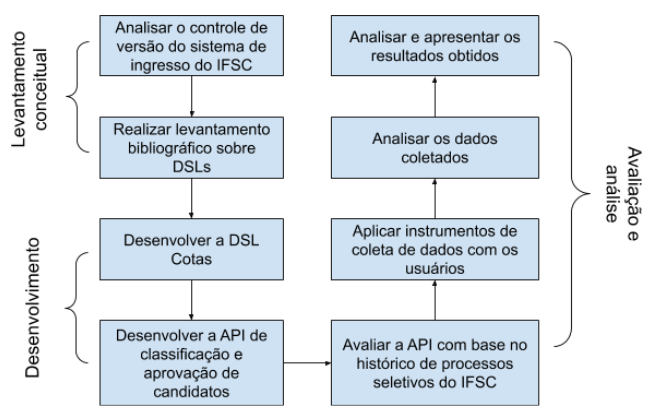
\includegraphics[width=0.76\textwidth]{chapters/metodologia/imagens/etapas.png}}

\par\medskip\textbf{Fonte:} Elaborada pelo autor (2020). \par\medskip

\end{figure}

    
    Com o intuito de apresentar os procedimentos metodológicos relativos ao ambiente da pesquisa, a Seção \ref{ambiente} descreve a metodologia de avaliação da DSL, abordando o perfil dos usuários, o detalhamento do exercício, o questionário aplicado e os critérios utilizados para avaliação da \gls{API}. 
    
    
    
  